\chapter{Proposed Application}

Below is a rough outline of the application and list of the development sprints for the application. More detailed descriptions of both the design of the application and the server side logic of the application are presented in later chapters. 

\section{Outline}

The outline of the application is as follows: 

The user starts the application by selecting a category of articles and their level of experience with German. From there, they are presented with a list of articles in that category, with each article having a difficulty rating. The user can then select an article based on the title of the article as well as the difficulty rating.

Once the user has selected the article, they are presented with the text of the article. From here, they can click on words in the article, and the application will show them a translation of the word and grammatical information about the word in a marginal gloss form. These gloss element can then be removed from the screen when no longer needed.

A marginal gloss was chosen as one of those is easier to implement than the other gloss presentation methods, while the decision to use dictionary level translations was made as they are effective and easier to implement than a more effective multimedia gloss.

A systems flow diagram of the basic outline of the application can be seen Figure \ref{fig:sf}

\begin{figure}
	\caption{Wireframe Mockup of the Category Input View}
	\label{fig:sf}
	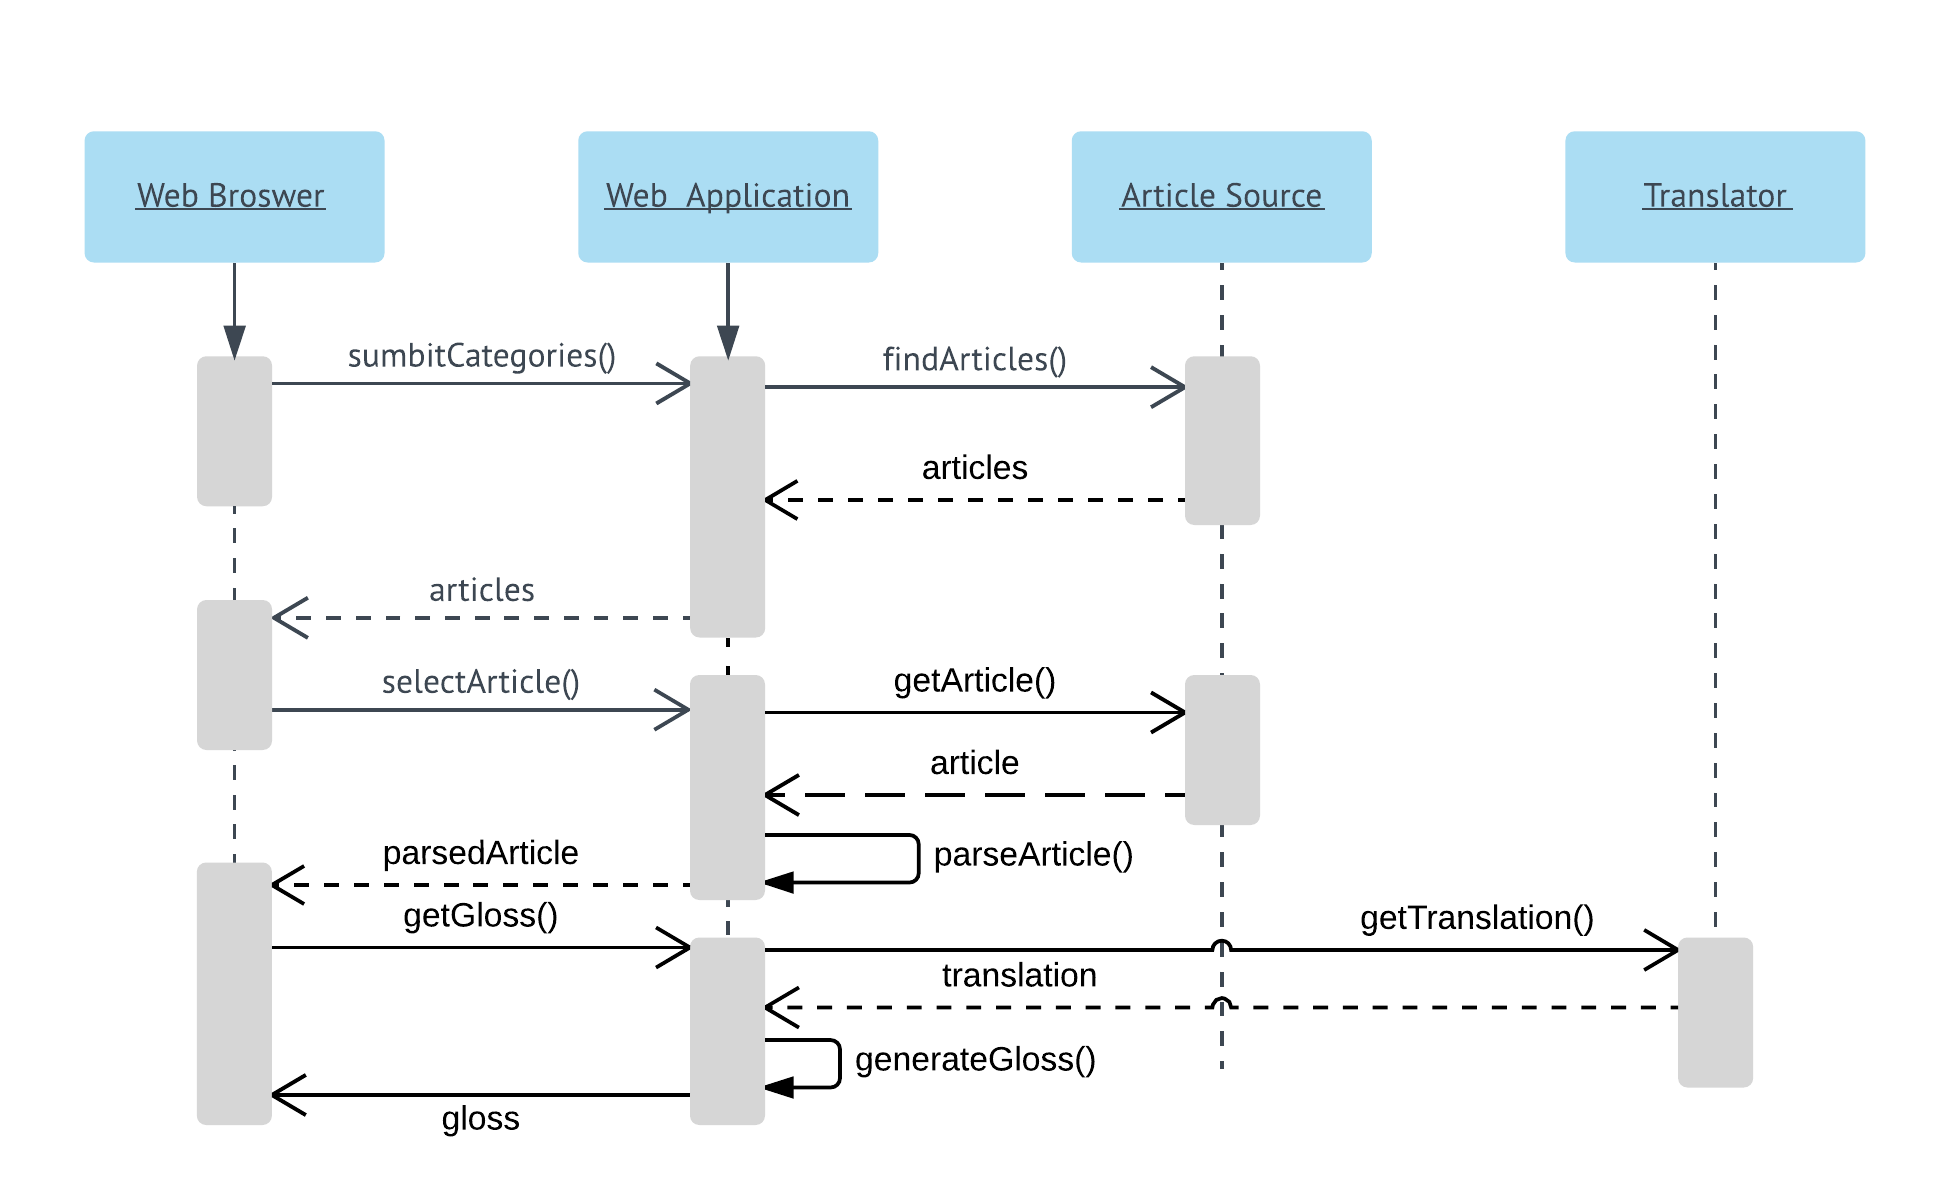
\includegraphics[width=\textwidth]{Graphics/SystemsFlow}
\end{figure}

\section{Development}

Development of the application was divided into six sprints and they were completed in the order in which they are described. The order was chosen as it would allow the application to reach minimal viable project status as soon as possible (end of Sprint 3), leaving the more advanced sprints for later. The sprints are detailed below.

\begin{enumerate}
	\item \textbf{Translation Lookup}
	
	The aim of this sprint is to establish a valid method to retrieve single word translation and grammatical data.
	
	\item \textbf{Article Parsing \& Presentation}
	
	The aim of this sprint is develop a method for the parsing of articles and then to present them through a web browser
	
	\item \textbf{AJAX}
	
	The aim of this sprint is to develop the JavaScript code that will allow the gloss to display entries.
	
	\item \textbf{Advance Parsing}
	
	The aim of this sprint is to allow advanced parsing methods to be performed on the text. Allowing for parts of speech identification of words. 
	
	\item \textbf{Article Discovery}
	
	The aim of this sprint is get the application to find articles on it's own, removing the need for the user to find their own articles.
	
	\item \textbf{Difficulty Rating System}
	
	The aim of this sprint it to develop the system that allows the application to rate how difficult the user will find various articles. 
	
\end{enumerate}
